
\section{Introdução}
Nesta secção é apresentada o estado da arte dos projetos realizados durante o estágio na empresa CapTemp. Nessa ordem é apresentado o funcionamento do sistema do Nidus desenvolvido pela empresa CapTemp e a sua página de configuração e visualização. Na secção \ref{Página do Coletor de Dados Nidus} são apresentadas também as metodologias e tecnologias que o sistema implementa atualmente para a compressão das páginas que dão suporte ao sistema. Na secção \ref{nbiot} e \ref{kea} irá ser introduzido o plano inicial dos projetos a desenvolver e a base já existente tal como as tecnologias que estes irão utilizar. Na secção \ref{solucoesDisponiveis} será abordado as soluções e tecnologias existentes na comunidade cientifica e alguns produtos similares, já existentes para os projetos anteriormente referidos.

\section{Coletor de Dados  - Nidus} \label{Coletor de Dados - Nidus}
\par
O sistema Nidus, apesar das suas diversas versões de hardware partilha entre todas as versões o mesmo centro de processamento o módulo RCM6760 da Rabbit. O sistema Nidus é composto por dois módulos principais, o Back-end que gere toda a parte de leitura de sensores, de atuação e envio de alertas, log entre as demais funcionalidades e o Front-end, duas páginas WEB Single-Application de modo a não sobrecarregar o módulo com a interface e mover o processamento da interface para o browser do cliente. Na primeira página é possível visualizar os valores obtidos pelo Back-end com atualização em tempo real. Na segunda página e possível carregar as configurações para realizar alterações nas mesmas. A comunicação entre os dois componentes é feita através de XML. Para consultar os valores na primeira página o Front-end acede ao ficheiro values.xml gerado no momento pelo Back-end onde contém todas os valores necessários. Na página de configurações á semelhança da primeira página os valores são carregados por um ficheiro XML o ficheiro setup.xml, incluindo a particularidade de aceitar pedidos POST de modo a alterar as configurações do equipamento.
\par A Nidus dispõe de base para o utilizador variadas funcionalidades tais como, leitura de sensores TH3 e Airo, INPUTS digitais, OUTPUTS digitais e analógico, leitura de sensores SNMP e MODBUS, envio de alertas via GSM e E-mail, programação de eventos, envio automático para um portal Cloud e Log Interno. Outras funcionalidades estão disponíveis mediante o pedido do cliente tais como sensores específicos, leitura de sensores por RS232 ou protocolos de comunicação específicos.
Na tabela \ref{tab0} são apresentadas as principais características do módulo RCM6760 da Rabbit.


\begin{table}[htb]
\centering
\caption{Especificações do Módulo RCM6760}\label{tab0}
    \begin{tabular}{|c|c|}\hline
  
Microprocessor&Rabbit 6000 \\\hline
Frequencia do Microprocessor  &200 MHz\\\hline
Flash Memory &4 MB (Código e Sistema de Ficheiros)\\\hline
SRAM&1 MB\\\hline
Power &260 mA  3.3V - Ethernet ON\\\hline
    \end{tabular}   
\end{table}

\subsection{Páginas do Coletor de Dados Nidus} \label{Página do Coletor de Dados Nidus}
\par
O código desenvolvido de modo a chegar á fase de produção é comprimido e compilado de modo a que ocupe o mínimo espaço e possa ser armazenado na memória do módulo e coabitar com o Firmware de Back-end, segue os seguintes passos de desenvolvimento:
\begin{enumerate}
\item Desenvolvimento/ alteração do código JavaScript necessário; 
\item Compressão das Imagens necessárias e posterior conversão em Base64 para incluir no JavaScript a imagem e o mesmo poder fazer a gestão da apresentação
\item Compilação/compressão do JavaScript num ficheiro único com recurso ao Google Clousure Platform, nesta etapa para cada versão de hardware é compilado consoante os ficheiros a incluir, poupando o espaço não necessário como o código referente aos Inputs e Outputs na Nidus C, C+ e W, ou o código referente ao módulo wireless nas versões não Wireless.
\item Geração do minificado do código HTML
\item Compressão de cada ficheiro para o seu respetivo GZIP
\end{enumerate}
\par
Após estes passos fica disponível uma nova versão da página pronta a ser carregada na Nidus.
Na imagem \ref{fignidusPage} é apresentado o estado e layout de uma página da Nidus IT no momento do inicio do estágio.

\begin{figure}[ht]
  \centering
  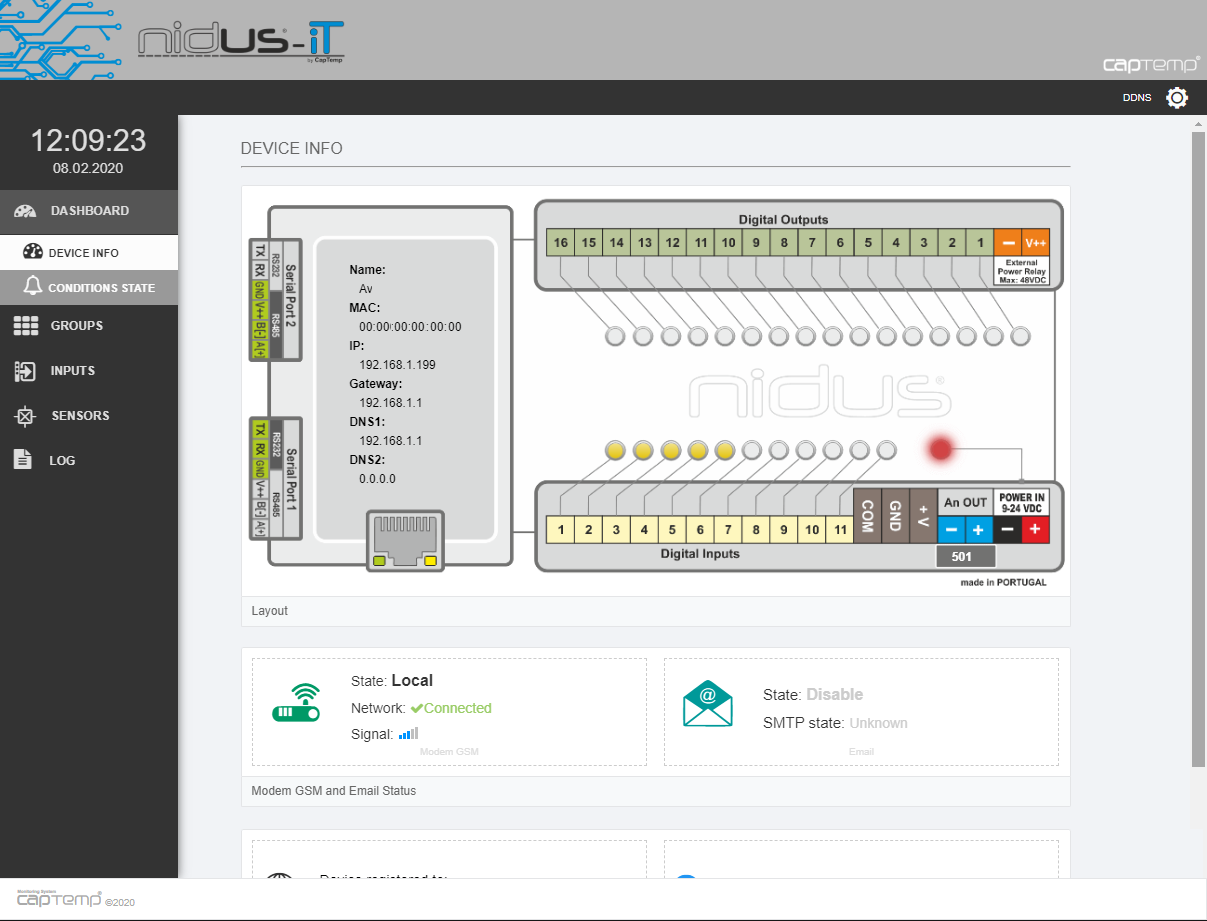
\includegraphics[width=0.75\textwidth]{images/layoutPAginaInit.png}
  \caption{Layout página da Nidus IT no início do estágio}\label{fignidusPage}
\end{figure}


\section {NB-Iot \& Digi Xbee 3 }\label{nbiot}
\par
Os módulos Xbee 3 da DIGI dispõe recentemente de uma versão NB-Iot/ LTE. Ideal para projetos com baixo volume de transmissão de dados e com gestão para economia da bateria. O módulo inclui também um compilador de Micropython, contundo a versão Micropython desenvolvida pela DIGE e incluída no módulo XBee, não inclui todas as funcionalidades do Micropyhton tais como por exemplo a biblioteca de gestão de Arrays e o módulo de "\_thread" pois o mesmo não tem suporte para multithread.
Na tabela \ref{tab1} são apresentadas as principais características do módulo XBee 3 da Digi\cite{Digixbee}.

\begin{figure}[ht]
  \centering
  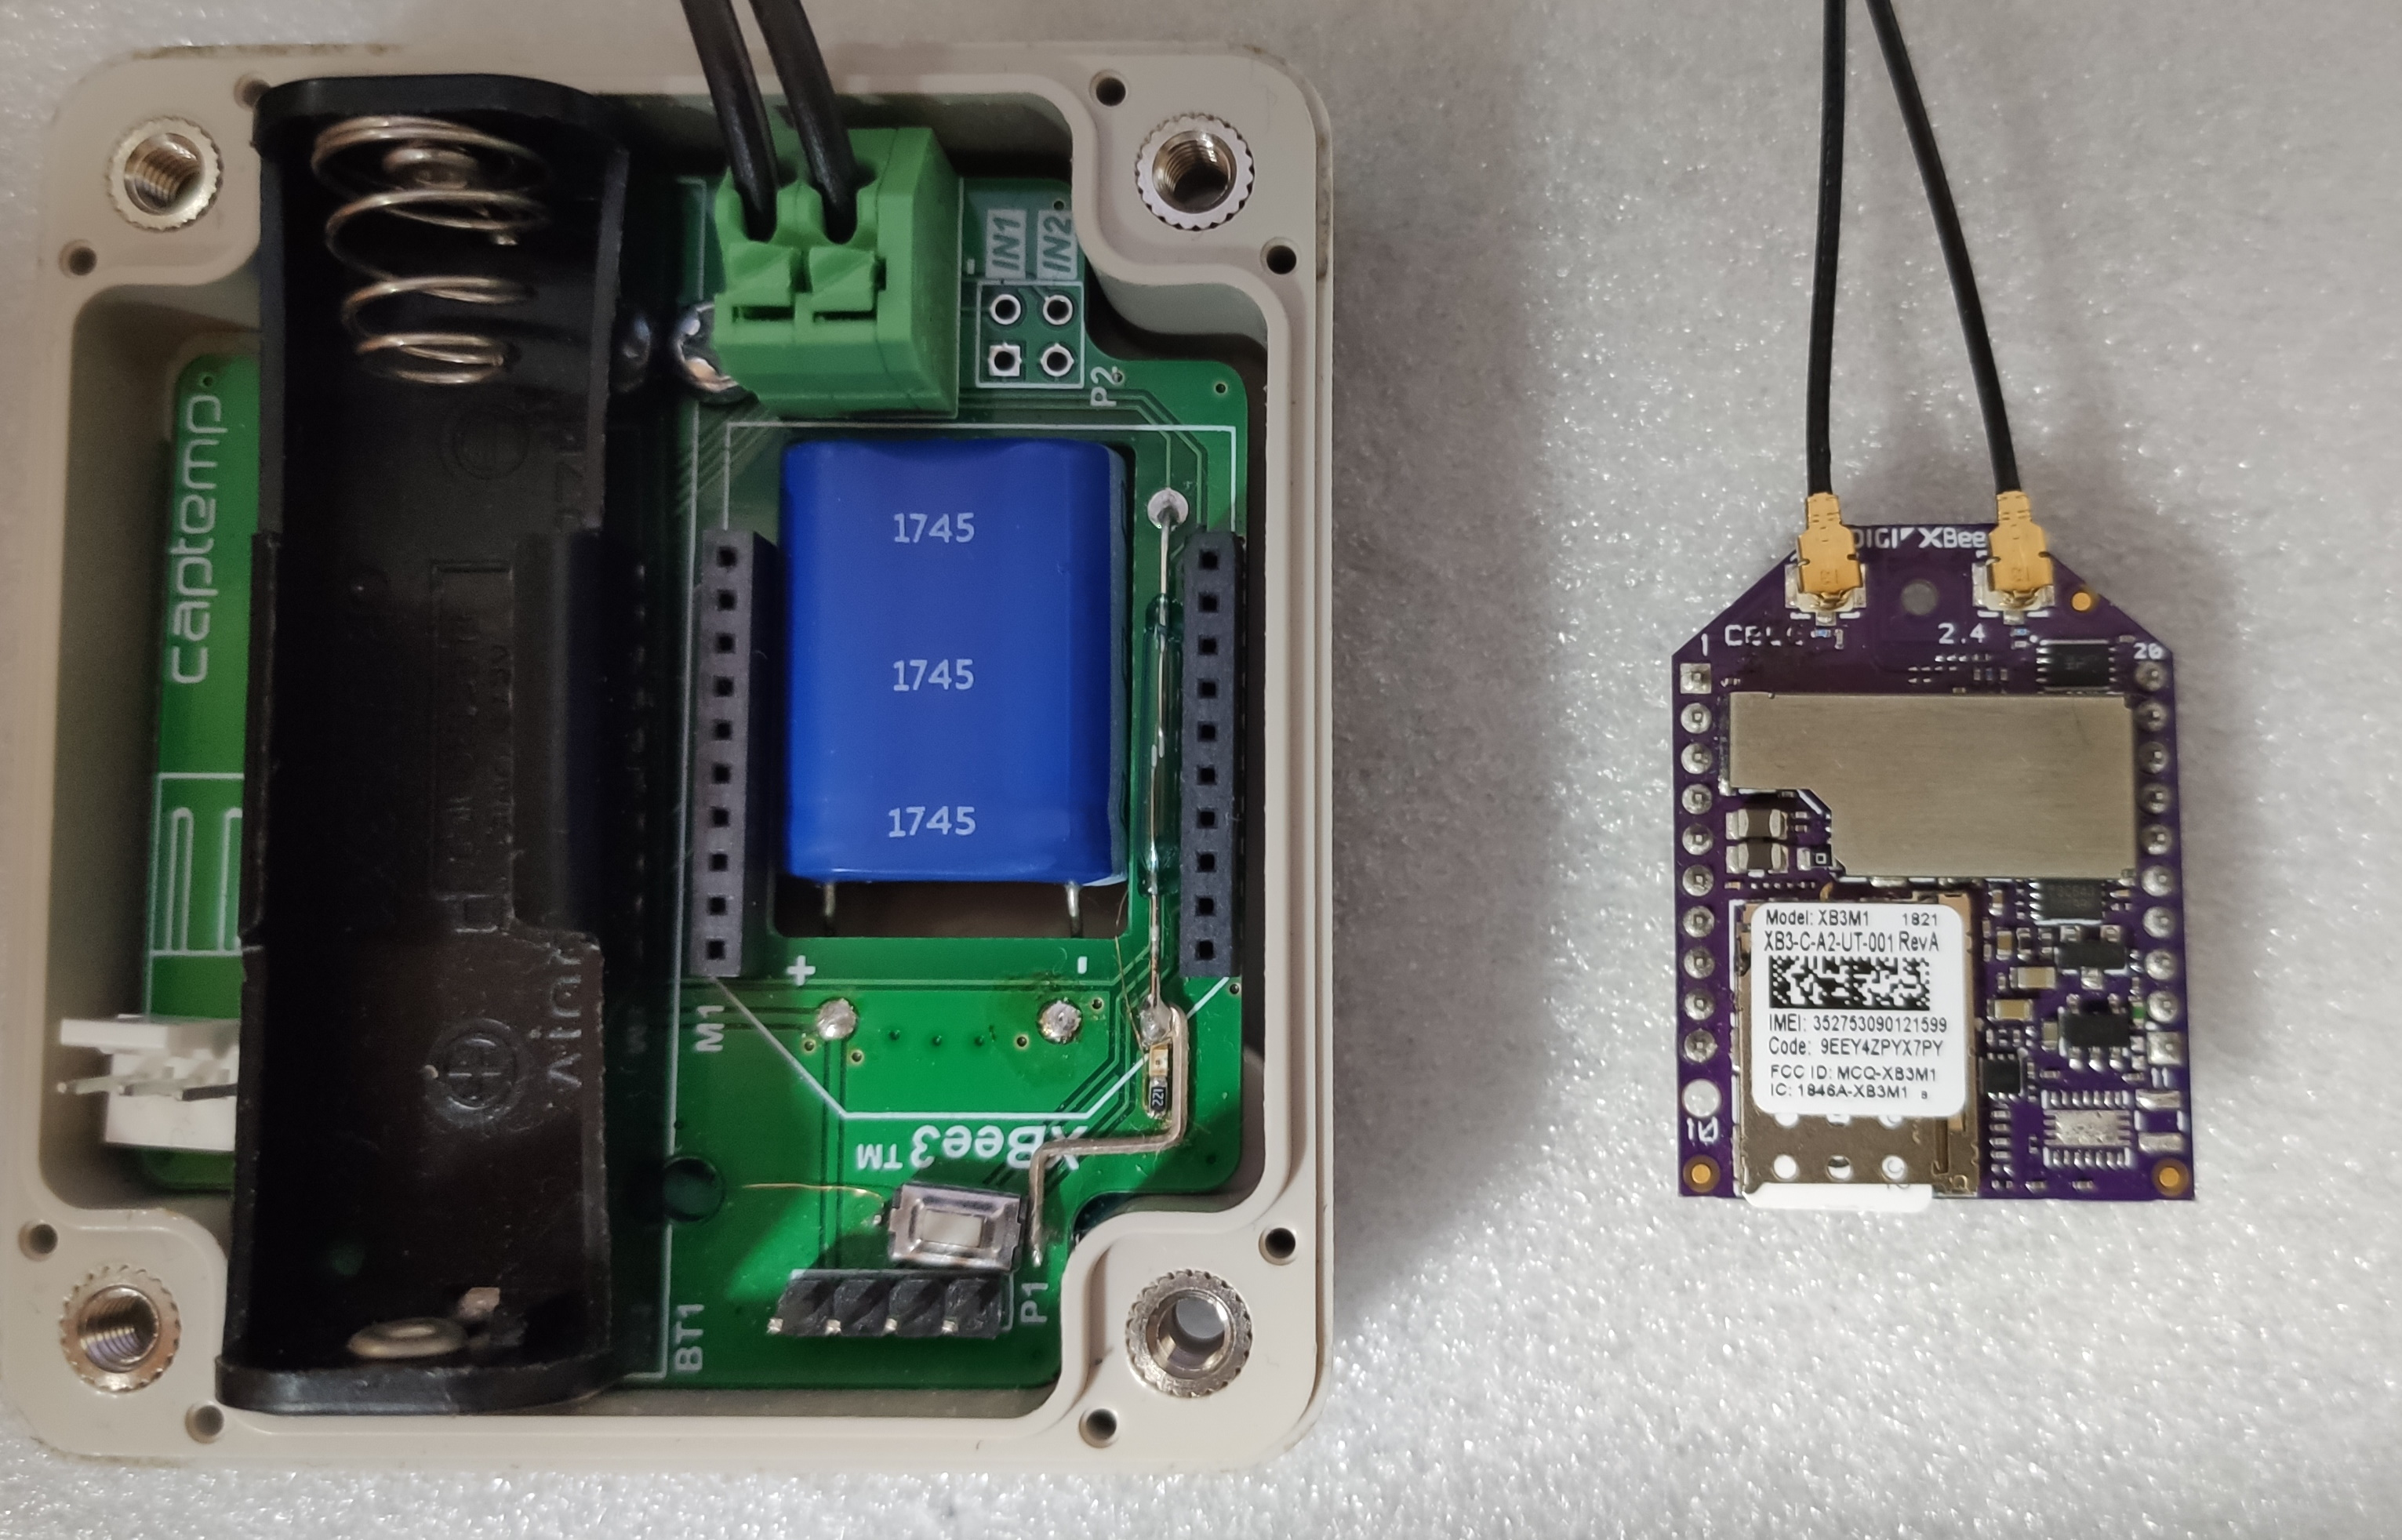
\includegraphics[width=0.45\textwidth]{images/xbee.jpg}
  \caption{Módulo Xbee 3 e placa de expanção}\label{figxbee}
\end{figure}

\begin{table}[htb]
\caption{Especificações do Módulo Xbee 3}\label{tab1}
\begin{tabular}{|c|c|}\hline
Chipset& U-blox SARA-R410M-02B\\\hline
Dimensões& 24.38 mm x 32.94 mm \\\hline 
Temperatura de Funcionamento& -40º C to +85º C \\\hline 
Tipo de SIM & 4FF Nano \\\hline
Interfaces& UART, SPI, USB \\\hline 
Programação MicroPython&  32 KB Flash / 32 KB RAM \\\hline 
I/O& 4 ADC (10-bit), 13 I/O digitais, USB, I2C \\\hline 
Bluetooth& BLE Ready \\\hline 
Potencia de Transmissão& Até 23 dBm \\\hline 
Sensibilidade de Receção (LTE-M) & -105 dBm \\\hline 
Sensibilidade de Receção (NB-IoT) & -113 dBm \\\hline 
Velocidade Downlink/Uplink(LTE-M) & Até 375 kb/s \\\hline 
Velocidade Downlink/Uplink(NB-IoT) & Até 27.2 kb/s Downlink, 62.5kb/s Uplink \\\hline 
Alimentação & 3.3-4.3VDC \\\hline 
Pico corrente na transmissão & \begin{tabular}{@{}c@{}} 550mA - Bluetooth OFF  \\  610mA - Bluetooth ON\end{tabular}\\\hline 
Corrente média de transmissão (LTE-M) & 235mA \\\hline 
Corrente média de transmissão (NB-IoT) & 190mA \\\hline 
Modo Power Save& 20uA \\\hline 
Modo Deep Sleep& 10uA \\\hline 
\end{tabular} 
\end{table}

\par A captemp pretende, através da utilização deste módulo e de uma placa de expansão desenvolvida pela própria, desenvolver uma versão do seu outro equipamento de Nb-Iot, mais simples representando numa opção de menor custo para o cliente. Será necessário desenvolver todo o código referente à gestão interna de Logs, o agendamento do envio e leituras e a otimização da memória e bateria. Sempre com recurso á programação em MicroPython.

\subsection {MicroPython}
\par O MicroPython\cite{MicroPython}, lançado em 2014, é um compilador e interpretador que implementa a linguagem Python3 e otimiza o seu funcionamento em microcontroladores. Escrito em C e disponibilizado em Open-Source é possível adaptar o mesmo para os diversos equipamentos. \par
É suportado por diversas arquiteturas de processadores tais como:
\par
\begin{itemize}
\item x86
\item x86-64
\item ARM
\item ARM Thumb
\item Xtensa
\end{itemize}
\par
Em microcontroladores que suportem Multi-thread , não sendo o caso do módulo usado está disponível ao programador o módulo de "\_thread" para criar processamento paralelo. Disponibiliza a programação de interrupções físicas, uteis em microcontroladores,  tem disponível um "Garbage collector" para gerir a memória do microcontrolador e bibliotecas tais como "usocket" para criação e gestão de sockets, "network" para gerir a comunicação com o módulo especifico de cada microcontrolador, ou a biblioteca para gerir o módulo de Bluethooth denominada por "ubluetooth"\cite{micropython_lib}. 

\subsection {NB-Iot/ LTE-M}
O NB-Iot ou Narrowband Iot é uma tecnologia de Low Power Wide Area.É indicado para sistemas Smart em diversas áreas como a monotorização, a agricultura, localizadores entre outras áreas. Similar á rede móvel mas para equipamentos com menor transmissão de dados e que não tem acesso a fontes de alimentação fixas e requerem de baterias, o NB-Iot promete autonomias das baterias a rondar os 10 anos\cite{u_2017}.Devido ao baixo volume de dados o plano de dados é possivel apenas com pequeno investimento obter anos e até decadas de transmissões da dados. De entre as vantagens podem-se destacar:
\begin{itemize}
\item Baixo Consumo
\item Longo alcance e boa penetração
\item Baixo custo de desenvolvimento na implementação da cobertura
\item Custo reduzido pelas transmissões
\item Sem necessidade de Roaming
\end{itemize}
\par
A cobertura da rede está a ser implementada pelas operadoras de telecomunicações que já possuem cobertura da rede GSM infrastrutura de ligação á rede Internet desenvolvida e apenas necessitam de 
disponibilizar cobertura nas antenas de rede móvel. É aconsellhado pelas operadoras que se utilize o Nb-Iot para equipamentos fixos e o LTE-M para equipamentos em movimento.

\subsubsection { Low Power Wide Area}
As redes Low Power Wide Area são redes usadas frequentemente no IOT quando é necessário enviar dados a distâncias longas.Combinam a largura de banda e o consumo de bateria presenete em redes como BLE e Zigbee, com alcance igual ou superior ás redes de comuniação GSM. São caracterizadas por ter longo alcance, um baixo custo e baixo consumo, onde simples baterias podem fornecer alimentacação na ordem das décadas. Este alcance pode ser conseguido por exemplo por redes multihop ou modulações especificas que privilegiem o consumo energético e o alcance. A comunicação 2G e 3G pode ser usada em comunicação M2M mas as mesmas tem uma largura de banda superior ao necessário o que resulta em consumo de bateria excessivo onde não é tirado proveito da largura de banda disponivel. Alguns exemplos de redes  Low Power Wide Area , ou simplesmente denominadas por LPWAN, são o DASH7, o SigFox, LoRa,  Ingenu, Telensa ou o NarrowBand Iot.\cite{lpwanoverview}

\begin{figure}[ht]
  \centering
  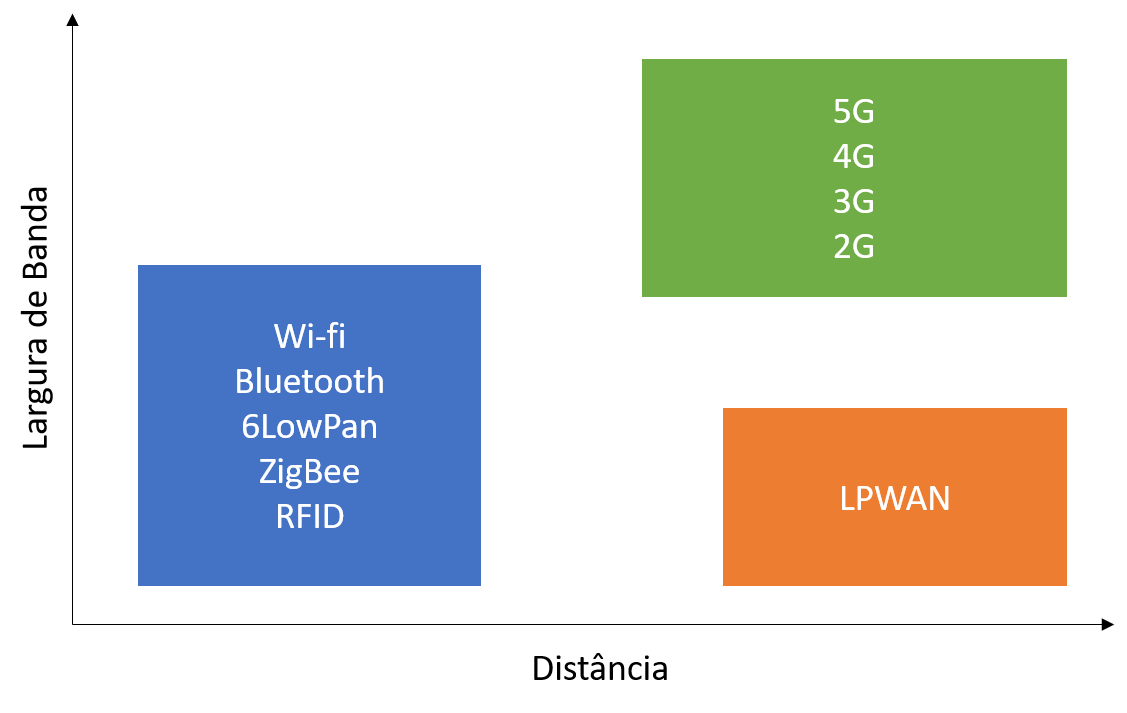
\includegraphics[width=0.45\textwidth]{images/lpwan.png}
  \caption{Gráfico com relação Distancia vs Largura de Banda\cite{masterthesisLPWAN}}\label{figgraphlpwan}
\end{figure}



\section {Kea Tracker}\label{kea}
O Projeto Kea Tracker utiliza Beacon’s da Ruuvi, uma Beacon open-source\cite{ruuvi}, que disponibiliza de forma open-source tanto o  Firmware para alterações, como as aplicações para Android e IOS. Será utilizada a aplicação disponibilizada alterando para o nosso funcionamento e o Firmware para disponibilizar a funcionalidade de data-logger.
\subsection{Beacons BLE}
\par
O Bluetooth Low Energy ou simplesmente BLE foi desenvolvido a pensar nos novos equipamantos IOT, onde os utilizadores querem vários equipamentos ligado ao mesmo tempo. Para tal foi desenvolvido o BLE que permite mais ligações ao mesmo tempo comparadamente ao Bluetooth clássico.
Como é indicado no nome, o principal fator diferenciador nesta versão, utilizada muitas vezes em equipamentos iot devido ao baixo consumo de aproximadamente metade relativamente ao Bluetooth normal. Outras caracteristicas melhoradas a visar os equipamentos de IOT no BLE são a baixa largura de banda e o baixo tempo de transmissão.

Com o desenvolver do BLE foram criados novos tipos de equipamentos, nomeadamente as beacons, equipamentos quase sempre alimentados por pilhas que comunicam através de BLE, tornando o equipamento portátil.As beacons são caracterizadas por transmitir pequenas quantidades de informação em broadcasting.
Existem dois tipos de beacons as beacons não connectaveis e as connectáveis. Como indicado no nome as beacons connectáveis permitem que um equipamento(como um smartphone) se connecte á beacons e esta fica preparada para receber dados. As não connectáveis apenas permitem o broadcasting dos dados, poupando energia pois apenas é necessário ter o módulo acordado para fazer o broadcast e o restante do tempo podem estar num estado sleep. Na figura \ref{blepacket} é apresentado o pacote que é transmitido em broadcast para os outros equipamentos receberem.

\begin{figure}[ht]
  \centering
  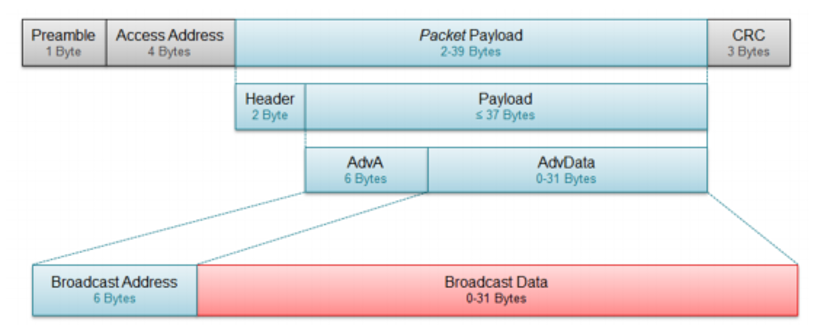
\includegraphics[width=0.95\textwidth]{images/blepacket.png}
  \caption{BLE Broadcast packet\cite{blepacket}}\label{blepacket}
\end{figure}


\subsection{Ruuvi Beacons}
\par Neste projeto o firmware das beacons apenas necessita de uma alteração, tornar a beacon numa beacon  connectável e esta armazenar internamente as ultimas leituras numb buffer circular e criar um data-logger e caso o cliente pretenda poderá connectar mais tarde para fazer o download para aplicação e posterior envio para o Senslive, não necessitando a proximidade so smartphone á beacon durante todo o tempo. A Ruuvi dispõe de dois modos de desenvolvimento do firmware da beacon em C ou usando o Espruino, á semelhanca do MicroPython um interpretador de JavaScript para microcontroladdores lançado em 2012, totalmente compativel com as Beacons da Ruuvi.
\subsection{Apps Smartphones}
Na fase inicial será adaptada a versão disponibilizada para Android para possibilitar a integração com o portal Senslive. A aplicação base disponibilizada pela Ruuvi foi desenvolvida em Kotlin\cite{ruuviappgithub}, uma linguagem desenvolvida pela JetBrains multiplataforma e que inclui o Android nessas plataformas compatíveis.
 De seguida estão apresentadas algumas alterações necessárias na aplicação:
\begin{itemize}
\item Alteração das Imagens e Logotipo da App;
\item Alteração do Nome da App;
\item Remoção de conteúdo não necessário;
\item Bloqueio do URL de envio para o portal Senslive;
\item Melhoramento da posição GPS;
\end{itemize}


\section{Soluções e Tecnologias Disponíveis} \label{solucoesDisponiveis}
	%alterar o metodo de compressa gzip para outro
	%comprimir as imagens
	%otimizar codigo

{\color{red} \rule{\linewidth}{0.5mm} } 
alternativas ao Gzip
\par
compressao de imagens
\par
tecnicas otimizaçao codigo
\par
produtos similares
\par
{\color{red} \rule{\linewidth}{0.5mm} } 








